Im Jahr 2002 hat es in Dresden extremes Hochwasser gegeben (siehe Abb. \ref{fig1}). Eine Maßnahme für den Hochwasserschutz besteht im Anlegen von Rückhaltebecken. 

Berechnen Sie für zwei nachfolgend beschriebene Szenarien näherungsweise das jeweils erforderliche Volumen. Verwenden Sie dafür das folgende mathematische Modell für die Durchflussgeschwindigkeit an der Messstelle Dresden:

$$v(t)=\frac{4500}{1+0,16t^2}+100$$

Dabei steht $t$ für die Zeit in Tagen und $v(t)$ für die Durchflussmenge in $\text{m}^3/\text{s}$ steht. An der Stelle $t=0$ befindet sich das Maximum  der Kurve. Finden Sie auch eine Veranschaulichung der berechneten Volumina.

\begin{enumerate}[label=(\roman*)]

\item Szenario 1: Begrenzung der Durchflussgeschwindigkeit auf $1710\, \text{m}^3/\text{s}$ (die im Zeitraum $t=-3,3..3,3\,\text{d}$
überschritten wurde).

\item Szenario 2: Begrenzung der Durchflussgeschwindigkeit auf $333\, \text{m}^3/\text{s}$ (die im Zeitraum $t=-10,7..10,7\,\text{d}$
überschritten wurde).

\end{enumerate}

Hinweis: Bei der Integration ist auf die Einheiten zu achten. $\int \frac{1}{x^2+1}$d$x=$atan$(x)+C$

\begin{figure}[ht]
	\centering
  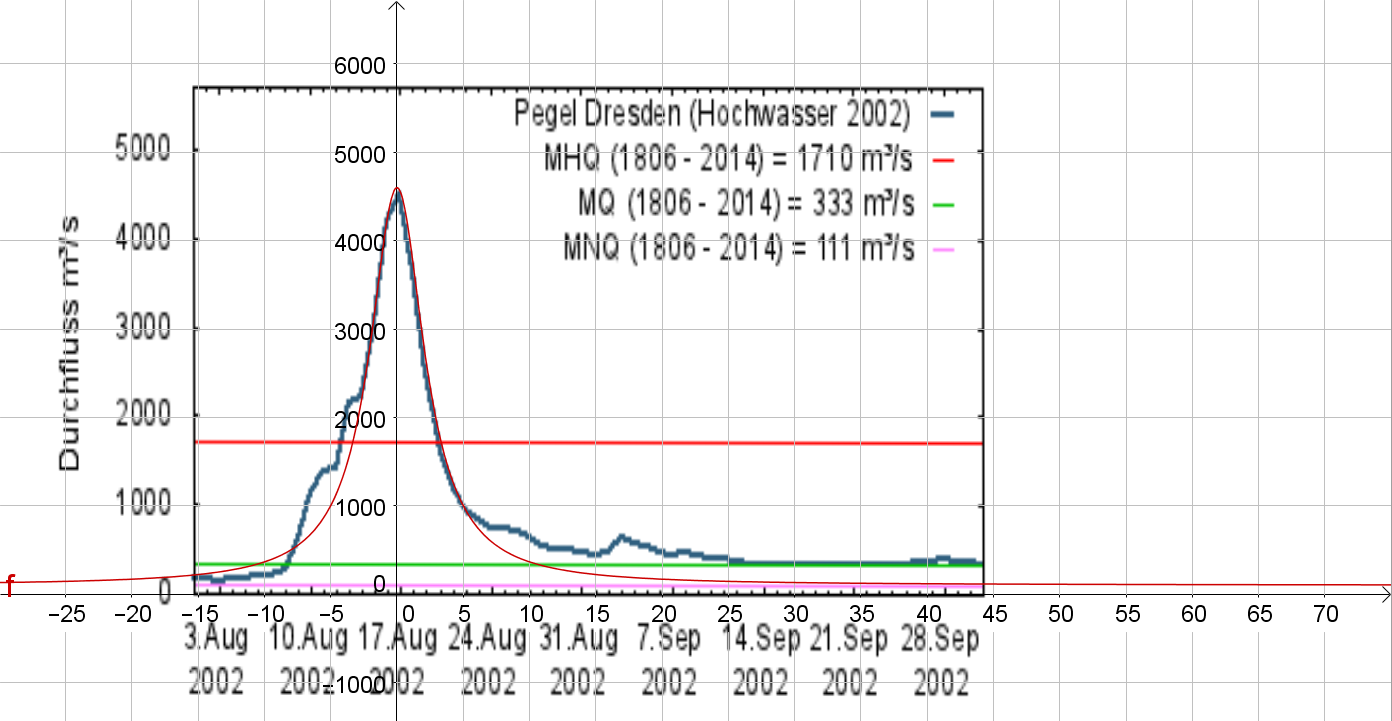
\includegraphics[width=0.65\textwidth]{../tex-snippets/ex-fn-model-1-img-a.png}
	\caption{Durchflussdaten zum Hochwasser des Jahres 2002 in Dresden mit Modellkurve; MHQ: Mittlerer Hochwasserabfluss, MQ: Mittlerer Abfluss, MNQ: Mittlerer Niedrigwasserabfluss in betrachteter Zeitspanne }
	\label{fig1}
\end{figure}

